%%%%%%%%%%%%%%%%%%%%%%%%%%%%%%%%%%%%%%%%%%%%%%
%% Template Thesis DGH UW v3.0
%%
%% Vincent Labatut 04/2015
%% Grégoire Lurton 07/2015
%%
%% v1   - 10/2014 : forme de rapport très différente
%% v2   - 02/2015 : modèle complètement refait
%% v2.1 - 03/2015 : définition de la page de titre
%% v2.2 - 03/2015 : correction de quelques bugs
%% v2.3 - 04/2015 : page de titre complétée (date, adresse postale, long titre)
%% v3.0 - 07/2015 : adaptation de la page de titre pour UW DGH
%% v3.1 - 07/2015 : inclusion de packages pour equations et test pour compilation knitr
%%%%%%%%%%%%%%%%%%%%%%%%%%%%%%%%%%%%%%%%%%%%%%
\documentclass[a4paper,11pt,final,twoside]{article}

%%%%%%%%%%%%%%%%%%%%%%%%%%%%%%%%%%%%%%%%%%%%%%%%%%%
%% Loading Packages
%%%%%%%%%%%%%%%%%%%%%%%%%%%%%%%%%%%%%%%%%%%%%%%%%%%
\usepackage[english]{babel}
\usepackage[utf8]{inputenc}
\usepackage[T1]{fontenc}
\usepackage{mathpazo}
\usepackage{eulervm}
\usepackage[top=2.5cm, bottom=2.5cm, left=2.5cm, right=2.5cm]{geometry}
\usepackage{setspace}
\usepackage[colorlinks=true]{hyperref}
\usepackage[french]{varioref}
\usepackage{lastpage}
\usepackage{fancyhdr}
\usepackage[table]{xcolor}
\usepackage{lmodern}
\usepackage{amsmath,amsthm,amscd,amssymb}
\usepackage{eulervm}

\usepackage{tikz}
\usetikzlibrary{decorations.pathreplacing , chains , intersections}

\usepackage{pgfgantt}
\usepackage{pgfcalendar}

%%%%%%%%%%%%%%
\tikzset{
>=stealth',
  punktchain/.style={
    rectangle,
    rounded corners,
    % fill=black!10,
    draw=black, very thick,
    text width=10em,
    minimum height=3em,
    text centered,
    on chain},
  line/.style={draw, thick, <-},
  element/.style={
    tape,
    top color=white,
    bottom color=blue!50!black!60!,
    minimum width=8em,
    draw=blue!40!black!90, very thick,
    text width=10em,
    minimum height=3.5em,
    text centered,
    on chain},
  every join/.style={->, thick,shorten >=1pt},
  decoration={brace},
  tuborg/.style={decorate},
  tubnode/.style={midway, right=2pt},
}


%%%%%%%%%%%%%%%


\usepackage[numbers]{natbib}
\bibliographystyle{apa-good}

%%%%%%%%%%%%%%%%%%%%%%%%%%%%%%%%%%%%%%%%%%%%%%%%%%%
%% Paper's Information -- TO TWEAK
%%%%%%%%%%%%%%%%%%%%%%%%%%%%%%%%%%%%%%%%%%%%%%%%%%%
%TITLE
\newcommand{\reporttitle}{Problems in HMIS in Developing Countries}

%AUTHORS
\newcommand{\reportauthors}{Grégoire Lurton}

%PROGRAM
\newcommand{\program}{PhD in Global Health}

%TRACK
\newcommand{\track}{Metrics Track}

%%%%%%%%%%%%%%%%%%%%%%%%%%%%%%%%%%%%%%%%%%%%%%%%%%%
%% Formatting stuff
%%%%%%%%%%%%%%%%%%%%%%%%%%%%%%%%%%%%%%%%%%%%%%%%%%%
\setlength{\headheight}{13.6pt} % due to a warning
\newcommand{\HRule}{\rule{\linewidth}{0.5mm}}
% Espace entre les paragraphes

% Headers and Footers
\pagestyle{fancy}
\fancyhf{}

\renewcommand{\headrulewidth}{0.4pt}
\renewcommand{\footrulewidth}{0.4pt}

\cfoot{\thepage}
\fancyhead[L]{\reporttitle}
\fancyhead[R]{\rightmark}

%%%% Define custom colors
\definecolor{grisclair}{rgb}{0.7,0.7,0.7}
\definecolor{grisfonce}{rgb}{0.5,0.5,0.5}
\definecolor{vert}{RGB}{74,171,67}

%%% PDF Metadatas
\hypersetup{
    pdftitle={\reporttitle},
    pdfauthor={\reportauthors},
    pdfsubject={\reporttitle},
    bookmarksnumbered=true,bookmarksopen=true,
	unicode=true,colorlinks=true,linktoc=all,
	linkcolor=blue,citecolor=blue,filecolor=blue,urlcolor=blue,
	pdfstartview=FitH
}

%%% Font  - Get sans serif
\renewcommand{\familydefault}{\sfdefault}


% Get Bulleted Lists Working
%\renewcommand{\FrenchLabelItem}{\textbullet}

\begin{document}
%%%%%%%%%%%%%%%%%%%%%%%%%%%%%%%%%%%%%%%%%%%%%%%%%%%
%% Title Page
%%%%%%%%%%%%%%%%%%%%%%%%%%%%%%%%%%%%%%%%%%%%%%%%%%%
\phantomsection
\begin{titlepage}
	\begin{tikzpicture}[remember picture,overlay]
		\node at (current page.south west)
			{
            \begin{tikzpicture}[remember picture,overlay]
 				\pgftext[x=0cm,y=25.37cm,bottom,left]{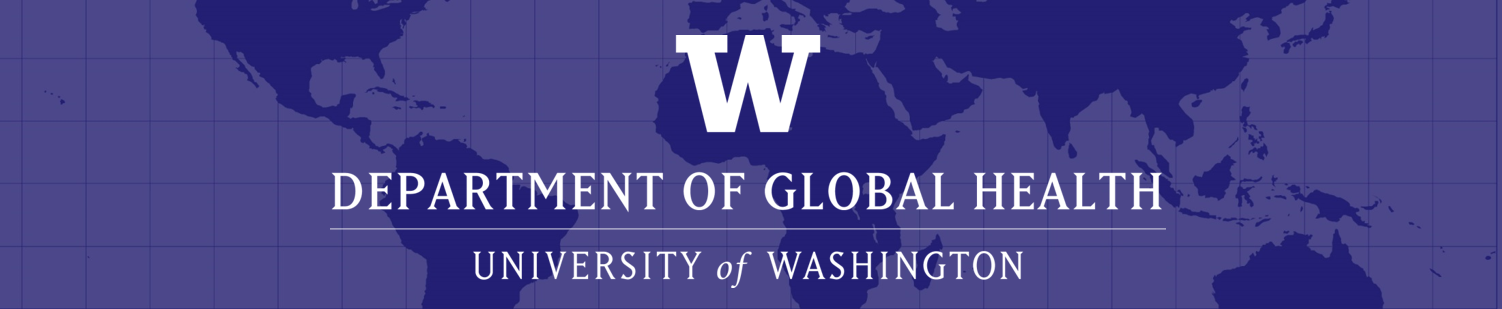
\includegraphics[width=21cm]{images/dgh_banner.png}};
 				\pgftext[x=1.1cm,y=24cm,bottom,left]{\fontsize{20}{20}{\textbf{\program}}};
 				\pgftext[x=1.1cm,y=23.2cm,bottom,left]{\fontsize{18}{18}{\textbf{\textcolor{grisfonce}\track}}};
 				\pgftext[x=10.5cm,y=16.5cm,bottom,center]{\fontsize{30}{30}{\textbf{Problems in HMIS \\ in Developing Countries}}};%\reporttitle
 				\pgftext[x=10.5cm,y=15.5cm,bottom,center]{\scalebox{0.77}[1]{\fontsize{20}{20}{\fontfamily{phv}\selectfont{}\textcolor{grisfonce}{\reportauthors}}}};
 				\pgftext[x=5.5cm,y=13.1cm,bottom,left]{\scalebox{0.6}[1]{\fontsize{18}{18}{\fontfamily{phv}\selectfont{}\textbf{\today}}}};
 				\pgftext[x=1.1cm,y=1.8cm,bottom,left]{
\includegraphics[width=6cm]{images/ihme_logo.png}};
                \pgftext[x=17cm,y=1.8cm,bottom,left]{
\includegraphics[width=3cm]{images/hai_logo.png}};
                \fill[fill=grisclair] (21cm,1cm) rectangle(0cm,0cm);
	\end{tikzpicture}
				};
			\end{tikzpicture}

\end{titlepage}

%% Get the page after title empty
\pagenumbering{gobble}% Remove page numbers (and reset to 1)
\newpage\null\thispagestyle{empty}\newpage








%%%%%%%%%%%%%%%%%%%%%%%%%%%%%%%%%%%%%%%%%%%%%%%%%%%%%%%%%%%%%%%%%%
%%%%    	FRONT MATTER
%%%%%%%%%%%%%%%%%%%%%%%%%%%%%%%%%%%%%%%%%%%%%%%%%%%%%%%%%%%%%%%%%%
\thispagestyle{plain}
\pagenumbering{roman}
\setcounter{page}{1}



\paragraph{Abstract}

The way I approach HMIS design is through a common differentiation of four main functions : data collection, data management, data analysis and data use. My overall hypothesis is that current approaches to HMIS in sub-saharan Africa build systems that overly relying on data collection and underinvest in other functions, thus building systems that rely on frontline health workers, who have other roles to fill, while specialized personals at district and national levels are performing trivial operations. These systems are thus  mainly geared towards their reporting functions, neglecting patient care functions, and are by design inefficient for either of these functions.

In my dissertation, I would like to explore tools and approaches that can correct the imbalance of these systems. I plan on working on 4 papers, one for each function of the HMIS :
\begin{enumerate}
\item	Data collection : I am working on an evaluation of the impact of the implementation of an EMR in HIV clinics in 341 hospitals in Kenya on the quality of care, and the ability of reporting to HIV program
\item	Data management : I am also currently working with the designers of OpenRBF to design a way to implement interoperability between OpenRBF and DHIS2. We have a designed a strategy for semantic interoperability between systems, and I will be testing this system in different settings and work on organizational interoperability.
\item	Data analysis : I plan on using HMIS data from different countries to test algorithms for facility performance monitoring based on reporting data.
\item	Data use : One of the reasons of the flow in current HMIS is for me the fact it is based on a function of administrative statistic thought as being justificative (workers presenting their results) and disciplinary (as a way to norm and supervise workers activity). This has been describe by Arjun Appadurai in the case of the production of statistics in colonial India, and is reinforced by an evolution of public statistics towards an evaluative value, as described by Alain Desrosières. I’d like to think on how these conditions of use of HMIS data are influencing the way the systems are thought and built, and how modifying this approach could help improve HMIS performances.
\end{enumerate}


% Table des matières
\cleardoublepage
% Dans le cas du recto verso, ajoute une page blanche si besoin
\phantomsection
\tableofcontents
\addcontentsline{toc}{section}{Table of Content}
\newpage
\addcontentsline{toc}{section}{\listfigurename}
\listoffigures
\newpage
\addcontentsline{toc}{section}{\listtablename}
\listoftables

\thispagestyle{fancy}

% Justification moins stricte : des mots ne dépasseront pas des paragraphes
\sloppy

%%%%%%%%%%%%%%%%%%%%%%%%%%%%%%%%%%%%%%%%%%%%%%%%%%%
%%%% 	MAIN MATTER
%%%%%%%%%%%%%%%%%%%%%%%%%%%%%%%%%%%%%%%%%%%%%%%%%%%

%% Set page numbering right
\cleardoublepage
\pagenumbering{arabic}
\setcounter{page}{1}

%% And Now get Writing !
\section{Introduction}

\subsection{Information in health systems}

Importance de l'information dans les systemes organises [edgar morin]
Importance historique dans le developmment des systemes de sante


"Les outils statistiques permettent de découvrir ou de créer des êtres sur lesquels prendre appui pour décrire le monde et agir sur lui" - citation sur la decision rationnelle. mais on sait que c'est un construit. Social et technique. Cas spécifique, statistique sanitaire.3


%% mettre ca dans l'approche methodologique
\textbf{tension entre valeur de l'etat et de la science se retrouve jouer à plein dans les HMIS ie HMIS sont objets composites. On veut montrer l'ambivalence de SI comme objet technique et politique. L'appproche utilisée pour les HMIS se fait surtout en termes de standardisation, et de précision croissante au niveau de la collecte de données. Approche critique des systèmes d'information. Réflexion se fait à la rencontre entre approche Science Studies et sciences humaines, et les avancées en science de l'information / statistique / Artificial Intelligence. Using multiple approaches, we wish to be able to defend a vision of HMIS that maximizes value of data collected and analyzed, by defending an approach centered on producing value at local level of health systems, and depending on non standardized processes at higher levels of hte health system to produce value and use data.}

We will do so pursuing three aims related to how
\begin{description}
    \item[Aim 1] Evaluate benefits of improving data collection techniques on the care of patients
    \item[Aim 2] Define a method for ensuring interoperability of different data systems commonly in HMIS
    \item[Aim 3] Analyze data with innovative approaches for monitoring of health services performance
    \item[Aim 4] Provide a broad historical and political analytical framework on how HMIS have been formalized and implemented in selected countries to understand how hmis are thought and conceived by health officials
\end{description}


decrire c'est gérer . role de description et de prescription

construction d'un espace politique d'équivalence et de codage



The use of statistical information in the design, the implementation and the evaluation of public policies is of growing interest in different domain of public life. Different trends in the thoughts and traditions of public life have led to this strengthened importance.

The improvement and the diffusion of tools and resources available for the production of public statistics have certainly be a first trend that has led to a better availability and use of data for decision making. In the meantime, the culture surrounding the production and use of numerical data in modern societies has evolved, both in reaction to increased capabilities of measurement, and of evolution of political and management sensibilities in these societies.

The use of data for pubic decision is consubstantial to the apparition and the development of public as a domain of public action. The "invention of population" in the second half of the XVIIIth century was made possible by the reform and development of demographic information in Europe and the development of demographic methods. In later stages, the development of sampling and inferential statistics methods in the XIXth century was also key to the targeting of specific public health interventions.

The use of data for policy making is thus, as we see, a combination of data sources, statistical methods, and political or social norms, that will define the conditions of utilisation of statistical evidence for policy making. Finding the proper data source, being able to analyze it and incorporating the results of this analysis in a political process is essential to the proper use and utilization of information systems.

In Global Health realm, the use of data for the definition of \textit{evidence based} intervention and policies has emerged as a panacea of project design and management. There are nonetheless difficulties in this regard. The global nature of public health means that statistical data available for analysis is by nature scattered and varied in nature, technical characteristics, quality and scope. In the meantime, the exigence of Global Health practitioners is to use and understand varied data sources in a unified global framework. The Global Burden of Disease initiative is a good example of this exigence of a global assessment of a wide variety of data from multiple contexts.

The challenge of using and processing different kinds of data varies with the nature of the data sources. The design and definition of survey data, for example, is governed by methodological and technical constraints that are comparable between settings and implementations. Meanwhile, data from health systems will be influenced by multiple factors, ranging from the administrative traditions in which they develop, to the level of resources involved in the design and building of these data systems, and to the type of activities performed in these systems. Among them, hospital data could arguably be considered the most impacted by these different factors.

\subsection{Importance of Health Management Information Systems}

%% Importance specifique des systemes de donnees hospitaliers
%% pb principal : peuvent pas etre penses avec utilisation en tete
%% enjeu est d'inventer la facon d'utiliser les donnes qui sortent des hmis
%% dans les pvd : enjeu supplementaire est la faible qualite des donnees diponibles

Among different data sources Health Management Information Systems (HMIS) are specific in so far as they are designed and thought, from the very beginning, to fulfill multiple purposes. If a survey is implemented, the only objective of its data collection tools is to collect data fitted to the sole purpose of completing the survey's objectives. In the meantime, HMIS typically rely on personals and resources whose primary goal is not the collection of data, but have other functions in the health system. This is also a difference with data stemming from sources specialized systems, like a survey implementations, for which every resource involved is aiming at producing quality data.

This non specificity and non specialization of HMIS is key to understand both its importance and its challenges. The overarching importance of Health Management Information Systems (HMIS) in modern health systems\cite{foundph} is as well recognized as the inability of most developing countries to implement well-performing HMIS. HMIS are important to provide information on the BIBLIO.

The low performance of HMIS comes from multiple origins. BIBLIO.

We contend that the difficulty of designing and implementing HMIS that deliver usable information for decision makers comes from technical difficulties, as well as from detrimental technical and organizational choices. HMIS are primarily considered functions of a health systems, and not as primarily statistical systems. As a result, in many situations, the logics and choices that are made in health systems are guided by administrative culture and the organization of health care in specific contexts, and are not primarily designed to perform as data systems. In this regard, HMIS are mainly aimed at very specific goals, limiting interoperability of systems and building systems that are not flexbile and are not designed to give information outside of a very limited, preset framework.

M\&E = version la plus degradee

data coll : qu'est-ce qu'on apprend de metadonnees. comment peut aider comprehension du fonctionnement
data man : interoperability, data management
data analyse : quelle approche innovante ? qu'est-ce qu'on peut lire ?
politique : le role du statisticien public


\paragraph{what is and what is not part of HMIS} The reasons for this weakness are as varied as HMIS are complex objects. Many functions are involved in developing and implementing an HMIS. There are different views that can be adopted to describe a HMIS. Some authors privilegiate the demand side of HMIS, by describing HMIS trough their end users and why they need information. Some authors will privilegy goals of a specific HMIS users. Some authors will concentrate on describing what should be included as being part of an HMIS. Finally some other actors will prefer to address different functions that are exerted inside of HMIS.

Even if the understanding of what should be considered part of a HMIS may vary depending on authors, every source regarding HMIS usually refers to the importance of using data for decision making at every level of health systems.

In the meantime, there is a role for HMIS in organizing work in health systems more widely, as the way data is collected has an impact on how work is organized inside health systems.

What are the main parts of HMIS ?SUBSYSTEMS : cf document liberia / openHIE : tous les differents composants d'un systeme d'information

Different uses ?

Questions asked are at multiple levels.

Desrosieres propose trois etapes du travail statistique :
    construction de classe d'equivalence
    Taxonomie
    Codage

On peut prendre cette lecture dans l'analyse des HMIS et les questions que l'on se pose.

HMIS mainly considered as a normative object in society. We contend this is not the only proper approach to it, and problematization can add benefits and create space for new solutions.


%% tiens plus de l'approche
%% ----------------------------------------------------------------------
Thinking about and working around HMIS requires different levels of thinking.

organizational : what makes an HMIS work, and what functions should
technological : right level of technology. adapt for best usage by different users (Illich)
analytical : what techniques of analysis to use with very specific data
political : how this data should be used to inform decisions ?

The objective of this proposal is to shape our angle of analysis in each of these approaches, and to identify research directions that will help furthering the understanding of HMIS in developing countries and offer solutions for currently important issues.
%% ----------------------------------------------------------------------

DISCUTER LA SPECIFICITE DES HMIS EN PVD VS PAYS DEVELOPPES  => approche historique.

We adopt a statistican's approach to HMIS.


\section{Conceptual framework - issues in HMIS designs}

	\subsection{Functional approach}
	\label{sec_function}

A first way to approach HMIS is to describe the principal functions that are necessary to have a HMIS to run. Figure \ref{HMISFunctions} presents a simplified sketch of the principal functions that are to be filled in any HMIS.

\begin{figure}[h]
\begin{center}
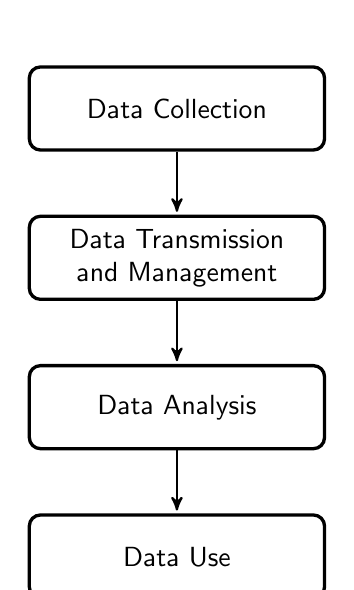
\begin{tikzpicture}[node distance=.8cm,  start chain=going below,]
     \node[punktchain, join] (DataCollection) {Data Collection};
     \node[punktchain, join] (DataManagement) {Data Transmission and Management};
     \node[punktchain, join] (DataAnalysis)   {Data Analysis};
     \node[punktchain, join] (DataUse) 		  {Data Use};
\end{tikzpicture}
\end{center}
\caption{Different functions inside the Health Information Systems}
\label{HMISFunctions}
\end{figure}

Four main functions can be found in HMIS.

\paragraph{Data Collection} Primary data collection is essential to the production of any information system. In the case of HMIS, data collection happens in health facilities, and is made by health professionals.

Data collected in facilities can be individual patient data collected in patients files or cards. It can also be a first level of aggregation of this data, as for indicators that are reported on a regular basis by facilities to higher levels of the health system. This reporting usually happen through standardized reports, and are then transmitted by successive aggregation to the top of the health pyramid.

\paragraph{Data Management} Data collected in health facilities has to be stored and archived, to be later accessed and reused. Data management work can encompass managing paper data, or managing computerized data. Individual patient data will be computerized in Electronic Medical Records (EMR) whereas aggregated indicators are stored in data-warehouses, of the type of the DHIS2 software.

\paragraph{Data Analysis} Data that is collected and stored in HMIS can then be analyzed. The type of analysis that is doable with EMR data will be different from the type of analysis that is possible to make with indicator type data.

\paragraph{Data Usage} What kind of decisions ? Memoire Cheickna.


	\subsection{Goal approach}
	\label{sec_goal}

Another approach to HMIS is a consideration of the stated goals of these information systems. Figure \ref{HMISGoals} shows what these goals are. The pyramidal representation of these needs is used to show that these goals fill data needs at different levels of health systems.

\begin{figure}[htp]
\centering
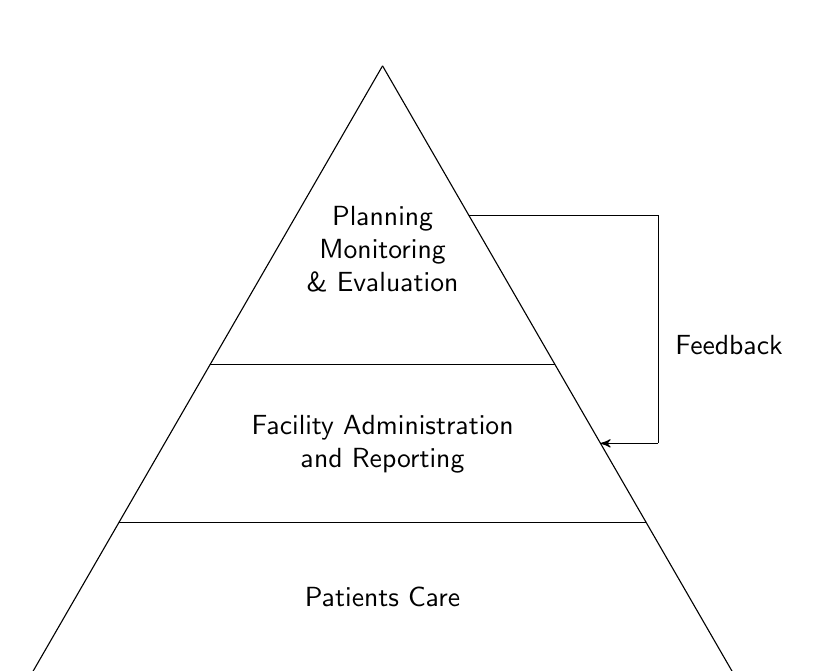
\begin{tikzpicture}[node distance=2cm]
\coordinate (A) at (-4.5,0) {};
\coordinate (B) at ( 4.5,0) {};
\coordinate (C) at ( 0,7.7942) {};
\draw[name path=AC] (A) -- (C);
\draw[name path=BC] (B) -- (C);
\draw (1.1,5.8971)--(3.5,5.8971) ;
\draw(3.5,5.8971)--(3.5,3) ;
\draw [->](3.5,3)--(2.77,3) ;
\node at (4.4,4.25) {Feedback};
\foreach \y/\A/\txtHigh in {0/Patients Care/0.8 ,2/Facility Administration \\ and Reporting/2.5,4/Planning \\ Monitoring \\ \& Evaluation /4.8}{
    \path[name path=horiz] (A|-0,\y) -- (B|-0,\y);
    \draw[name intersections={of=AC and horiz,by=P},
          name intersections={of=BC and horiz,by=Q}] (P) -- (Q)
          node[align = center,above] at (0,\txtHigh){\A};
          }
\end{tikzpicture}
\caption{Objectives of HMIS}
\label{HMISGoals}
\end{figure}

\paragraph{Patients Care} Taking care of patients is the primary goal of a health facility. To do so, it is necessary to collect data on these patient, data that will be transmitted (to other services), stored and reused during further follow-ups.

\paragraph{Facility Administration and Reporting} At facility level, HMIS data is used in daily activities to quantify and forecast needs in health inputs, and to create reports for higher levels of the health system.

\paragraph{Planning, Monitoring \& Evaluation } People in charge of the administration of health systems at local or national also need data to monitor activities in the health system, to evaluate the results of interventions, to report to funders or to plan later interventions.

\subsection{Problematization and problem analysis}

Using the framework we presented in sections \ref{sec_function} and \ref{sec_goal}, we identify important issues in the way HMIS are designed, implemented and used in developing countries. Our analysis is looking at the adequacy of HMIS methods and practices with the aims of these systems. We posit there is an overemphasis that is put on data collection in a lot of systems, which jeopardizes the way health information systems perform.

The reasons for this overemphasis can be traced to the intellectual frameworks that has surrounded the design and development of statistical systems in developing countries, and the evolution of what collecting data for organizations means.

\subsubsection{The administrative legacy}

There has been a long term evolution since the early XIXth century as of how data should be produced and used in health systems. As


reductio ad M\&E


Question de la statistique coloniale. Les différents niveaux de la statistique administrative, importance de la justification et du contrôle dans l'utilisation faites des données administratives.

There is a primary problem in the use of HMIS data. Alain Desrosières has shown the richness and complication of the production and use of statistics in modern societies. Desrosières shows how two traditions have been cohabiting in the early ages of the production of social statistics\cite{admin_savant}.

\begin{quote}
"The first tradition is administrative, and is based on political science and the law, on the German Staatenkunde, from the time of Conring and Achenwall. It is more taxonomic than metrological: it is designed to classify facts systematically rather than measure them, which is the essence of the other tradition, the "English" tradition. The latter, inspired more by the natural sciences and by progress made in measurement and probability theories, is a distant relation of the English political arithmetic of Graunt and Petty."
\end{quote}

Desrosières later shows how these two traditions have bee reconciled in the modern figure of the statistician, at the same time administrator and scientist. It is useful to keep considering this tension when thinking about maturing statistical systems like developing countries' HMIS. Being able to distinguish between situations when actors of HMIS are acting as administrators, and when the position is that of a metrician is essential to understand HMIS issues and offer informed solutions.

This distinction is essential at many levels. The whole debate around the level of uncertainty that is bearable around a measurement is not only important for statisticians. Choosing a given approach will have an impact on how primary data will be collected, how it will be analyzed, and how it will be used. In many usages of HMIS, complete enumeration is deemed necessary, but this can be discussed. What is the level of confidence one can bear around the estimation of a stock of drugs ?

In other dimensions, how can civil society help for HMIS design and evaluation


\subsubsection{Three HMIS strategies}

Functions of HMIS (cf. section \ref{sec_function}) are not independent of each other. Defining the relative importance of different functions of HMIS in the overall systems can change greatly the way a HMIS functions, and the output it produces. We differentiate three paradigmatic types of HMIS, varying on the respective influence of different functions. Building on the idea that a HMIS is used to provide an image of the activities and performances of a health system, we describe each function as a different way of making an image.

\paragraph{Jigsaw Puzzle HMIS} - A common way to design HMIS in developing countries can be considered as a Jigsaw Puzzle approach. A series of indicators are designed by program managers. These indicators are deemed to be \textit{sensitive} and \textit{specific}, and are supposed to allow managers to track and identify precisely the performance of health systems, and to provide important information on health system's results. The HMIS will then be organized to produce carefully designed indicators at facility level, and to transmit these indicators to higher levels for aggregation.

In these types of system, a lot of importance given to data collection functions, as the quality of this primary data collection is key to the rest of the work in the system. Data management in these system is often limited to aggregating some data and transmitting it to different actors in the health systems. Data analysis is usually mainly descriptive and is limited to presentation of time series values or mapping of indicators along administrative boundaries.

These systems are similar to jigsaw puzzles, made of very specific pieces, to compose a predetermined picture. When they are well designed, these systems can provide very useful information on health systems. Meanwhile, they are very vulnerable to any variation in primary data collection. As for jigsaw puzzles having a piece missing will jeopardize the possibility to get the whole picture right.

\paragraph{Pixel HMIS} - Another way to conceive HMIS is built on the collection and use of a multitude of individual data collected through Electronic Medical Records (EMR). Once the data is collected, program managers can query different indicators on different levels of aggregation, that can be extracted from different EMRs. In the best situations, interoperability of multiple EMRs present in a country allow for a central analysis of the data \cite{pugliese2009large}.

These systems allow a great variety of analysis, with a great variety of approaches. Analysis can be led varying geographic and time focus, or changing definitions of computed quantities. It also allows longitudinal analysis that are more difficult to perform with other approaches.

This approach thus involves a great investment in primary data collection and management, and allows elaborate data analysis. Meanwhile, it requires a technological investment and maturity that is seldom achieved in rich countries, and thus is very rare in developing countries.

\paragraph{Tangram HMIS} - Between the two extremes that are puzzle and pixel HMIS,


Most of interventions to improve HMIS are geared toward improving \textit{data quality} or its availability, all characteristics that concern the data collection function. Meanwhile, facility reporting

Problème est l'équilibrage des différentes fonctions. Mauvaise articulation. Comment rééquilibrer.

Statistique publique

Non adptation de l'administration et des systèmes utilisés, comme montré dans le cas de l'algérie

Data collection should be the same for all the goals. Highly specialized data collection. Low specialization of other functions. This shows a bizarre profile. Data users everywhere. Very little data specialists.

\subsubsection{Data collection as most important function}

Our approach to HMIS relies on two premises. First, in resource limited health care systems, data collection tasks often rely on non specialized personnel, that has to cary out other tasks, such as taking care of patients or providing support services for the care of patients. HMIS tasks should be as simple as not to be detrimental to patients care.

Secondly, HMIS should be conceived as data systems at list as much health system functions. This means adapting a framework around HMIS that perceives HMIS mainly as a system that shadows other health system functions to collect data, and think of HMIS mainly as systems which primary goal to collect and analyse data, and should thus be optimized in this regard.

Holding these two premises in mind leads us to think and desing on methods that will be aimed at imrpoving the higher functions of HMIS, such as data management and data analysis, without putting an unwelcome data collection burden on actors of health systems. Our theory of change for HMIS is thus based on a strengthening of data management, data analysis and data usage in HMIS.

data collection improvements are strongly limited by current constraints whereas there is much more room for improvement in other functions.

Schema

Comment faire pour améliorer l'utilisation des données dans les systèmes de santé. Quels sont les aspects importants ?

Theory of change for HMIS ?


\begin{figure}[ht]
\begin{center}
\fbox{ 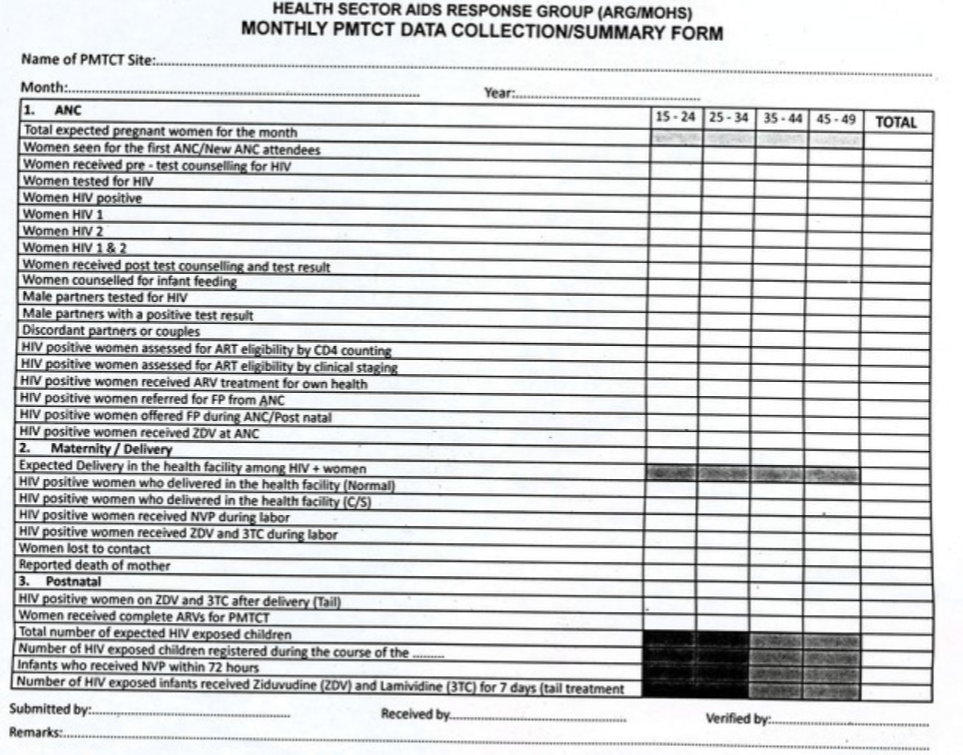
\includegraphics[scale=0.7]{figure/Picture1.png} }
\caption{Sierra Leone PMTCT registry (2012)}
\end{center}
\end{figure}

\section{Objectives}

	\subsection{Main objective}

Our main objective is to explore methods and approaches that can be used to improve the comprehension and the operations of HMIS in developing countries. Looking at different angles of HMIS, we aim at understanding how each of the different functions of HMIS can be leverage to improve the outcomes of HMIS operations.

The dissertation will be built in four parts, each part being a look at a specific function of HMIS. For each of these functions, we aim at providing a better understanding of the challenges met, or to offer solutions to improve outcomes of HMIS.

	\subsection{Specific aims}
	\subsubsection{EMR and individual health}

A first aim will be to understand how data collection itself impacts quality of care. As we postulate that data collection is not a neutral activity, we want to look into how primary data collected in HIV care setting can impact the outcome of care and organizational capabilities of HIV services. The case we will explore for this project is provided through a project implemented by ITech in Kenya.

\begin{figure}[ht]
\begin{minipage}{.4\textwidth}
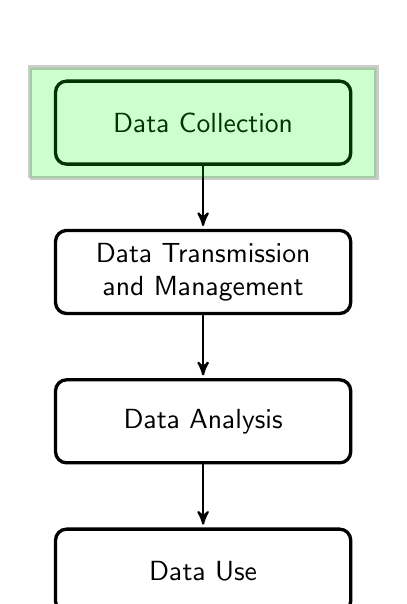
\begin{tikzpicture}[node distance=.8cm,  start chain=going below,]
     \node[punktchain, join] (DataCollection) {Data Collection};
     \node[punktchain, join] (DataManagement) {Data Transmission and Management};
     \node[punktchain, join] (DataAnalysis)   {Data Analysis};
     \node[punktchain, join] (DataUse) 		  {Data Use};
     \filldraw[ultra thick, draw=black, fill=green, opacity=0.2] (-2.2,-.7) -- (-2.2,.7) -- (2.2,.7) -- (2.2,-.7) -- (-2.2,-.7) ;
\end{tikzpicture}
\end{minipage}
\begin{minipage}{.5\textwidth}
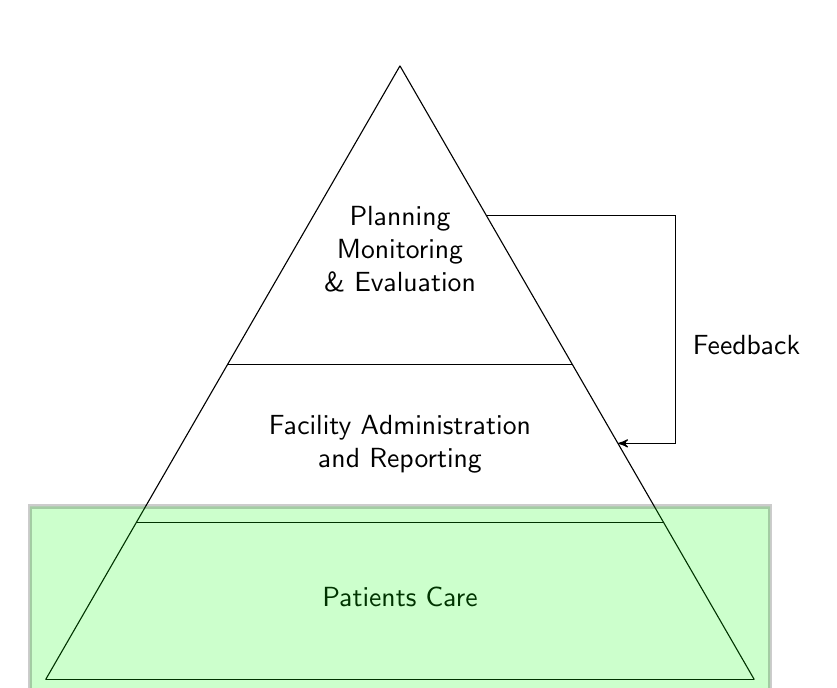
\begin{tikzpicture}[node distance=2cm]
\coordinate (A) at (-4.5,0) {};
\coordinate (B) at ( 4.5,0) {};
\coordinate (C) at ( 0,7.7942) {};
\draw[name path=AC] (A) -- (C);
\draw[name path=BC] (B) -- (C);
\draw (1.1,5.8971)--(3.5,5.8971) ;
\draw(3.5,5.8971)--(3.5,3) ;
\draw [->](3.5,3)--(2.77,3) ;
\node at (4.4,4.25) {Feedback};
\foreach \y/\A/\txtHigh in {0/Patients Care/0.8 ,2/Facility Administration \\ and Reporting/2.5,4/Planning \\ Monitoring \\ \& Evaluation /4.8}{
    \path[name path=horiz] (A|-0,\y) -- (B|-0,\y);
    \draw[name intersections={of=AC and horiz,by=P},
          name intersections={of=BC and horiz,by=Q}] (P) -- (Q)
          node[align = center,above] at (0,\txtHigh){\A};
          }
    \filldraw[ultra thick, draw=black, fill=green, opacity=0.2] (-4.7,-.2) -- (-4.7,2.2) -- (4.7,2.2) -- (4.7,-.2) -- (-4.7,-.2) ;
\end{tikzpicture}
\end{minipage}
\caption{Objective one definition}
\label{Paper One}
\end{figure}


\paragraph{Setting}

\paragraph{Data}

\paragraph{Analysis}

\paragraph{Timeline}

\begin{figure}[h]
\begin{ganttchart}[vgrid,hgrid]{1}{24}
\gantttitle{2016}{12}
\gantttitle{2017}{12} \\
\gantttitlelist{1,...,12}{1} \gantttitlelist{1,...,12}{1}\\
%\ganttgroup{Group 1}{1}{7} \\
\ganttbar{Data Extraction}{1}{3} \\
\ganttbar{Data Cleaning}{2}{4} \\
\ganttbar{Data Analysis 1}{5}{6} \\
\ganttmilestone{Sharing First Results}{6} \\
\ganttbar{Data Analysis 2}{7}{9} \\
\ganttmilestone{Sharing Final Results}{9} \\
\ganttbar{Paper Writing}{9}{11} \\
\ganttmilestone{Paper Submission}{11}
\end{ganttchart}
\caption{Gantt Chart for Paper 1}
\end{figure}


\subsubsection{Interoperability }

The second approach of this dissertation regards the management of data collected in hospitals in developing countries. Many systems have been developped to store this data and use it in different situations. Meanwhile, some problems are frequently found, that prevent statisticians and public health scientists to use this data.

One important limitation is the difficulty that different data management have to exchange data between each others. If interoperability (define interoperability) comes from different aspects, semantic interoperability appears to be one of the most challenging, as it involves actors who are not involved in technical / technological discussions but much more operate according to managerial logics. Thus, using data comming from different systems can be difficult when definitions are different, and one can have a hard time comparing data from different systems. Developing standards and method that can be used to ensure interoperability between systems is essential to liberating the potential of different data systems to inform decision making. -> TO MAKE ANALYSIS AND INFORM DECISION MAKING

\paragraph{Interoperability} POINT SUR INTEROPERABILITY BRAA / SAHAY

\paragraph{A flexible approach to interoperability}EXPLICATION TRAVAIL DEJA FAIT

\begin{figure}[ht]
\begin{minipage}{.4\textwidth}
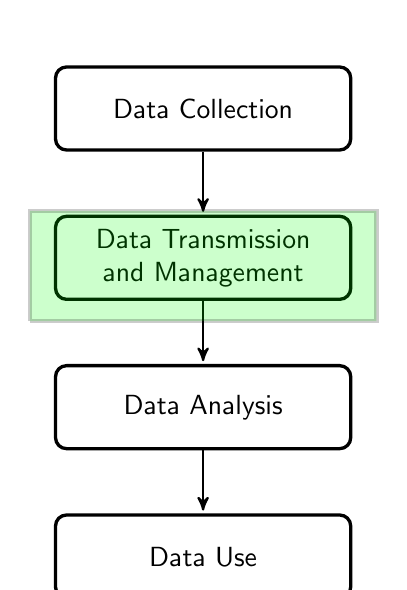
\begin{tikzpicture}[node distance=.8cm,  start chain=going below,]
     \node[punktchain, join] (DataCollection) {Data Collection};
     \node[punktchain, join] (DataManagement) {Data Transmission and Management};
     \node[punktchain, join] (DataAnalysis)   {Data Analysis};
     \node[punktchain, join] (DataUse) 		  {Data Use};
     \filldraw[ultra thick, draw=black, fill=green, opacity=0.2] (-2.2,-2.7) -- (-2.2,-1.3) -- (2.2,-1.3) -- (2.2,-2.7) -- (-2.2,-2.7) ;
\end{tikzpicture}
\end{minipage}
\begin{minipage}{.5\textwidth}
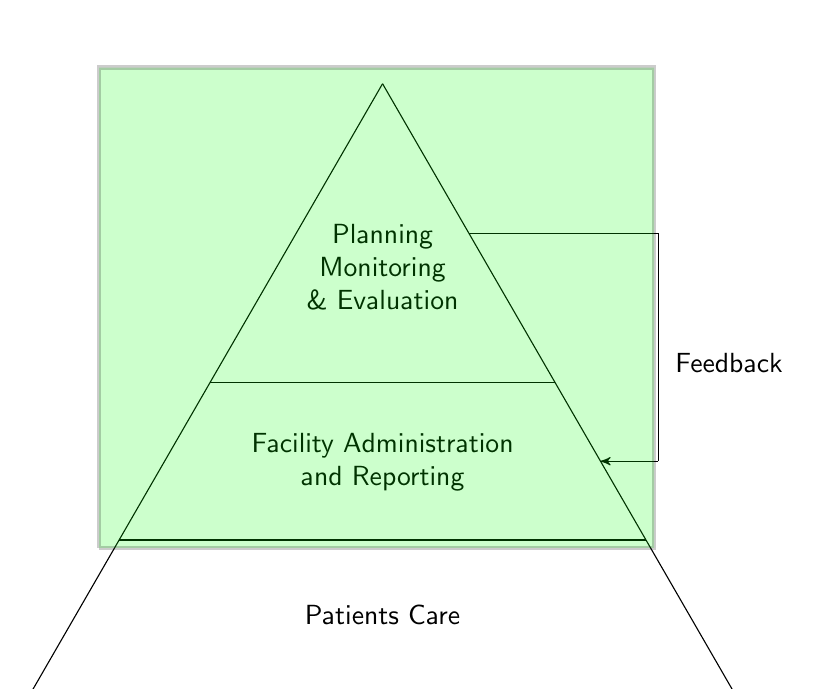
\begin{tikzpicture}[node distance=2cm]
\coordinate (A) at (-4.5,0) {};
\coordinate (B) at ( 4.5,0) {};
\coordinate (C) at ( 0,7.7942) {};
\draw[name path=AC] (A) -- (C);
\draw[name path=BC] (B) -- (C);
\draw (1.1,5.8971)--(3.5,5.8971) ;
\draw(3.5,5.8971)--(3.5,3) ;
\draw [->](3.5,3)--(2.77,3) ;
\node at (4.4,4.25) {Feedback};
\foreach \y/\A/\txtHigh in {0/Patients Care/0.8 ,2/Facility Administration \\ and Reporting/2.5,4/Planning \\ Monitoring \\ \& Evaluation /4.8}{
    \path[name path=horiz] (A|-0,\y) -- (B|-0,\y);
    \draw[name intersections={of=AC and horiz,by=P},
          name intersections={of=BC and horiz,by=Q}] (P) -- (Q)
          node[align = center,above] at (0,\txtHigh){\A};
          }
    \filldraw[ultra thick, draw=black, fill=green, opacity=0.2] (-3.6,1.9) -- (-3.6,8) -- (3.45,8) -- (3.45,1.9) -- (-3.6,1.9) ;
\end{tikzpicture}
\end{minipage}
\caption{Objective two definition}
\label{Paper Two}
\end{figure}

\paragraph{Setting} Plusieurs situations. comparer la performance. differents modes d'implementation.
Aspect politique ? mise en place d'un systeme par partie minimale utile.

\paragraph{Data}

\paragraph{Analysis} We aim at multiple end points :
\begin{itemize}
    \item What is a minimal actionable workload ?
    \item Can we guide the norming and tagging of indicators through machine learning approaches
    \item at the same time analytic and software problem
\end{itemize}

\begin{itemize}
    \item A set of
\end{itemize}

\paragraph{Timeline}


\subsubsection{Analysis}

Data from HMIS, when avalaible, is hard to analyze. A reason for this is the perceived weak quality of the data, and the high dimensinality of the collected data. Both these difficulties imply the need for at least some statistical approach of this data before it is used. We thus aim at defining a generic framework for statistical use of HMIS data, and at providing an example of how HMIS data could be use for facility quality benchmarking in a health system.

\begin{figure}[ht]
\begin{minipage}{.4\textwidth}
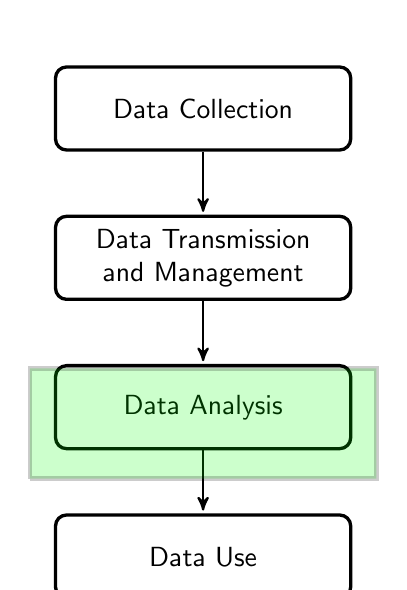
\begin{tikzpicture}[node distance=.8cm,  start chain=going below,]
     \node[punktchain, join] (DataCollection) {Data Collection};
     \node[punktchain, join] (DataManagement) {Data Transmission and Management};
     \node[punktchain, join] (DataAnalysis)   {Data Analysis};
     \node[punktchain, join] (DataUse) 		  {Data Use};
     \filldraw[ultra thick, draw=black, fill=green, opacity=0.2] (-2.2,-4.7) -- (-2.2,-3.3) -- (2.2,-3.3) -- (2.2,-4.7) -- (-2.2,-4.7) ;
\end{tikzpicture}
\end{minipage}
\begin{minipage}{.5\textwidth}
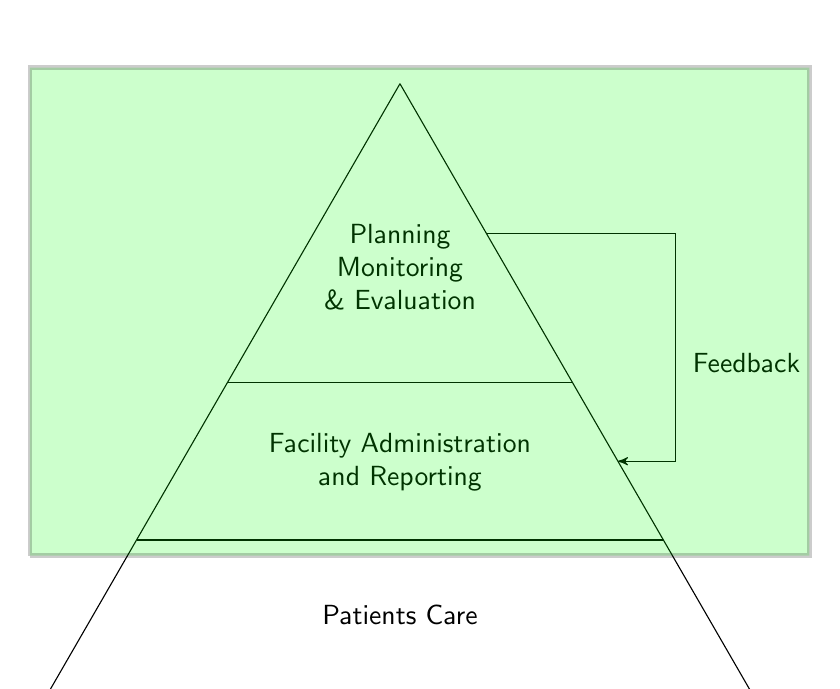
\begin{tikzpicture}[node distance=2cm]
\coordinate (A) at (-4.5,0) {};
\coordinate (B) at ( 4.5,0) {};
\coordinate (C) at ( 0,7.7942) {};
\draw[name path=AC] (A) -- (C);
\draw[name path=BC] (B) -- (C);
\draw (1.1,5.8971)--(3.5,5.8971) ;
\draw(3.5,5.8971)--(3.5,3) ;
\draw [->](3.5,3)--(2.77,3) ;
\node at (4.4,4.25) {Feedback};
\foreach \y/\A/\txtHigh in {0/Patients Care/0.8 ,2/Facility Administration \\ and Reporting/2.5,4/Planning \\ Monitoring \\ \& Evaluation /4.8}{
    \path[name path=horiz] (A|-0,\y) -- (B|-0,\y);
    \draw[name intersections={of=AC and horiz,by=P},
          name intersections={of=BC and horiz,by=Q}] (P) -- (Q)
          node[align = center,above] at (0,\txtHigh){\A};
          }
    \filldraw[ultra thick, draw=black, fill=green, opacity=0.2] (-4.7,1.8) -- (-4.7,8) -- (5.2,8) -- (5.2,1.8) -- (-4.7,1.8) ;
\end{tikzpicture}
\end{minipage}
\caption{Objective three definition}
\label{Paper Three}
\end{figure}

\paragraph{Setting}

\paragraph{Data}

\paragraph{Analysis}

\paragraph{Timeline}


	\subsubsection{Data Use}

Finally, recognizing even an excellent technical framework can not ensure the proper use of statistical information in a health system, we want to reflect on the culture of data use in developing countries health systems. To do so, we want to adopt a post colonial approach, and understand how a vision of statistics resulting from colonial rule and neo-liberal management results in a deficit of data using for health systems related decisions.

\begin{figure}[ht]
\begin{minipage}{.4\textwidth}
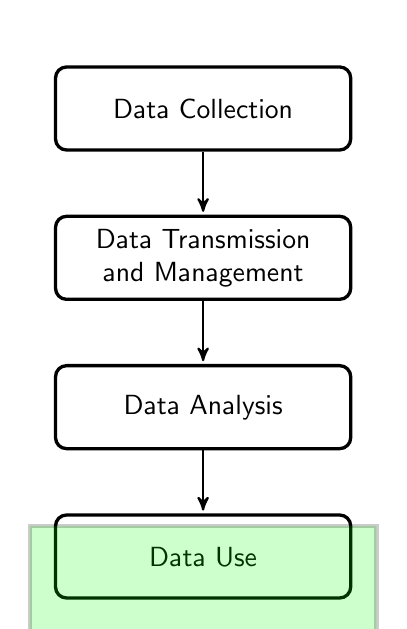
\begin{tikzpicture}[node distance=.8cm,  start chain=going below,]
     \node[punktchain, join] (DataCollection) {Data Collection};
     \node[punktchain, join] (DataManagement) {Data Transmission and Management};
     \node[punktchain, join] (DataAnalysis)   {Data Analysis};
     \node[punktchain, join] (DataUse) 		  {Data Use};
     \filldraw[ultra thick, draw=black, fill=green, opacity=0.2] (-2.2,-6.7) -- (-2.2,-5.3) -- (2.2,-5.3) -- (2.2,-6.7) -- (-2.2,-6.7) ;
\end{tikzpicture}
\end{minipage}
\begin{minipage}{.5\textwidth}
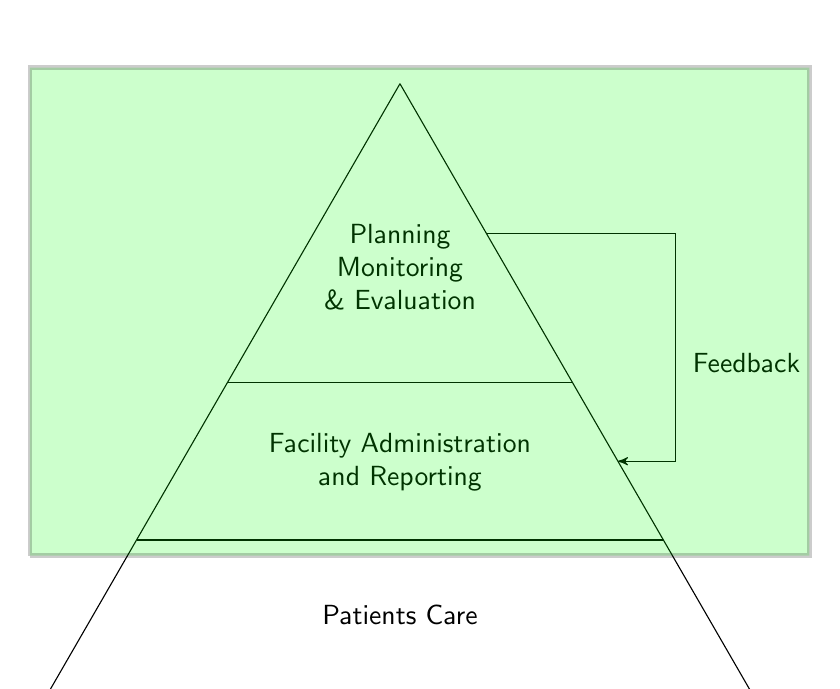
\begin{tikzpicture}[node distance=2cm]
\coordinate (A) at (-4.5,0) {};
\coordinate (B) at ( 4.5,0) {};
\coordinate (C) at ( 0,7.7942) {};
\draw[name path=AC] (A) -- (C);
\draw[name path=BC] (B) -- (C);
\draw (1.1,5.8971)--(3.5,5.8971) ;
\draw(3.5,5.8971)--(3.5,3) ;
\draw [->](3.5,3)--(2.77,3) ;
\node at (4.4,4.25) {Feedback};
\foreach \y/\A/\txtHigh in {0/Patients Care/0.8 ,2/Facility Administration \\ and Reporting/2.5,4/Planning \\ Monitoring \\ \& Evaluation /4.8}{
    \path[name path=horiz] (A|-0,\y) -- (B|-0,\y);
    \draw[name intersections={of=AC and horiz,by=P},
          name intersections={of=BC and horiz,by=Q}] (P) -- (Q)
          node[align = center,above] at (0,\txtHigh){\A};
          }
    \filldraw[ultra thick, draw=black, fill=green, opacity=0.2] (-4.7,1.8) -- (-4.7,8) -- (5.2,8) -- (5.2,1.8) -- (-4.7,1.8) ;
\end{tikzpicture}
\end{minipage}
\caption{Objective four definition}
\label{Paper Four}
\end{figure}



Reflections on social conditions of HMIS data usage  / politics of administrative statistics.

Data is not produced to create knowledge, but to implement disciplinary monitoring. Thinking mainly in terms of indicators.

Case study : analyse de textes M\&E / projets de reforme de systemes hmis, et analyse de la vision des HMIS qu'ils proposent. quelle place pour la societe civile ? inversion des priorites.

\paragraph{Setting}

\paragraph{Data}

\paragraph{Analysis}

\paragraph{Timeline}


%%%%%%%%%%%%%%%%%%%%%%%%%%%%%%%%%%%%%%%%%%%%%%%%%%%
%% 			BIBLIOGRAPHY
%%%%%%%%%%%%%%%%%%%%%%%%%%%%%%%%%%%%%%%%%%%%%%%%%%%
%\cleardoublepage
%\phantomsection\addcontentsline{toc}{section}{Références}
\newpage
\bibliography{bibliographie}


\end{document}
